\documentclass[aspectratio=169,10pt]{beamer}
\usetheme{Madrid}
\usepackage[T1]{fontenc}
\usepackage{lmodern}
\usepackage{tikz}
\usepackage{adjustbox}
\usepackage{array}
\usetikzlibrary{shapes.geometric,arrows.meta,positioning,calc,fit,backgrounds}

% Brand Color Palette matching PrismSpace theme
\definecolor{prismNavy}{RGB}{13,29,54}
\definecolor{prismBlue}{RGB}{38,126,190}
\definecolor{prismTeal}{RGB}{28,161,157}
\definecolor{prismMint}{RGB}{232,248,245}
\definecolor{prismGold}{RGB}{229,166,50}
\definecolor{prismDark}{RGB}{15,23,42}
\definecolor{prismIndigo}{RGB}{79,70,229}
\definecolor{prismSlate}{RGB}{71,85,105}
\definecolor{cardBg}{RGB}{248,250,252}

\setbeamercolor{frametitle}{bg=prismNavy,fg=white}
\setbeamertemplate{navigation symbols}{}
\setbeamertemplate{footline}{\hfill\textbf{PrismSpace} $\cdot$ CSE, CEK\hspace{1em}|\hspace{1em}\insertframenumber/\inserttotalframenumber\hspace{1.5em}\vspace{0.4em}}

\newcommand{\pk}[1]{\textbf{#1}}
\newcommand{\idx}[1]{\textit{#1}}
\newcommand{\comp}[1]{\texttt{#1}}

\begin{document}

\begin{frame}[t]{03. Browser Database Schema: \texttt{PrismDB} (Figure 4.4)}
\vspace{-0.35cm}
\centering
\adjustbox{max width=0.98\linewidth, max height=0.85\textheight}{%
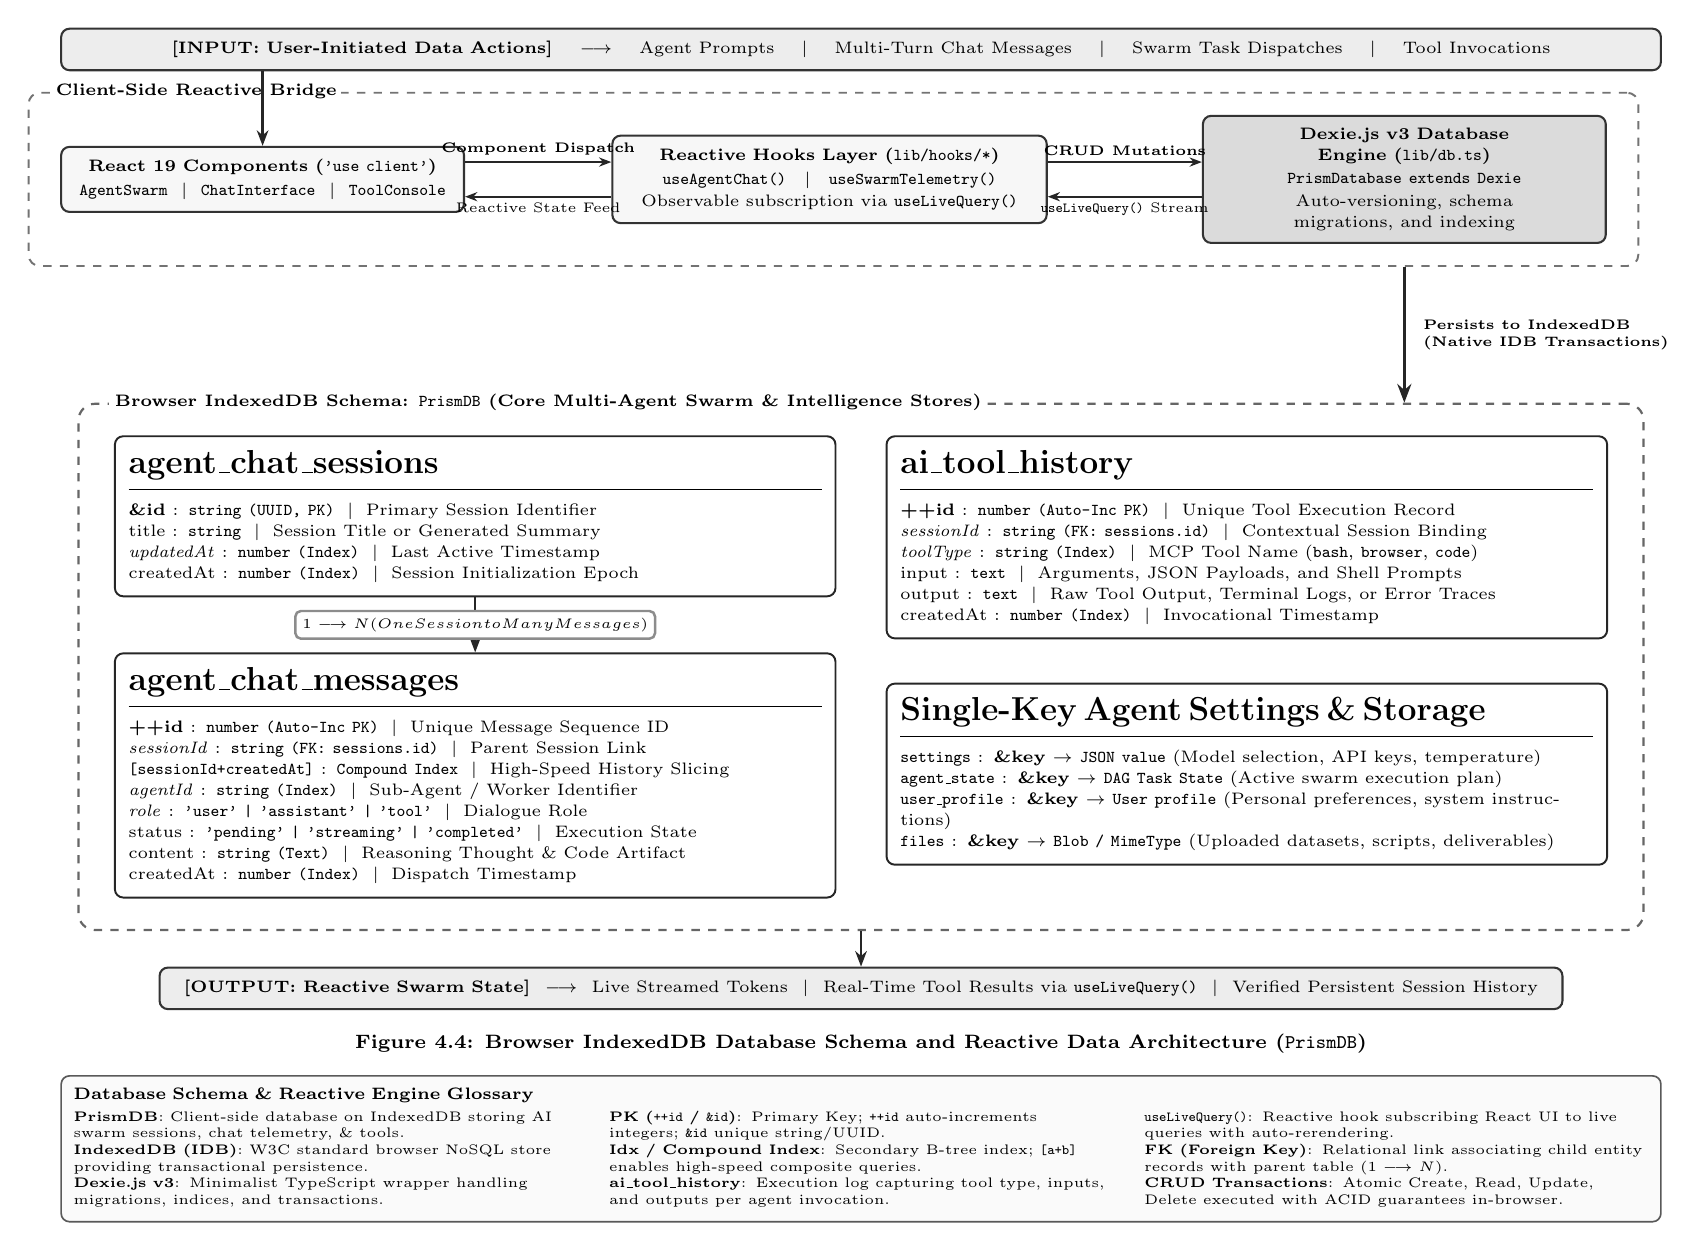
\begin{tikzpicture}[
    x=1cm, y=1cm,
    font=\sffamily,
    table/.style={
        rectangle,
        draw=black!85,
        line width=0.7pt,
        fill=white,
        rounded corners=3pt,
        inner sep=5pt,
        font=\fontsize{6.2}{7.6}\selectfont
    },
    system_box/.style={
        rectangle,
        draw=black!80,
        line width=0.75pt,
        fill=black!3,
        rounded corners=3pt,
        inner sep=4.5pt,
        align=center,
        font=\fontsize{6.0}{7.4}\selectfont
    },
    rel_arrow/.style={
        -{Stealth[scale=0.85]},
        line width=0.8pt,
        draw=black!85
    }
]

    % =========================================================================
    % 1. TOP: INPUT NODE (Core Multi-Agent Swarm Input Actions)
    % =========================================================================
    \node [system_box, text width=20.0cm, fill=black!7] (input_node) at (0, 7.4) {
        \textbf{[INPUT: User-Initiated Data Actions]} $\;\longrightarrow\;$
        Agent Prompts $\;\vert\;$ Multi-Turn Chat Messages $\;\vert\;$ Swarm Task Dispatches $\;\vert\;$ Tool Invocations
    };

    % =========================================================================
    % 2. MIDDLE: CLIENT-SIDE REACTIVE BRIDGE (Perfect clearance)
    % =========================================================================
    \node [system_box, text width=4.8cm] (react_ui) at (-7.6, 5.75) {
        \textbf{React 19 Components (\texttt{'use client'})}\\[0.15em]
        \texttt{AgentSwarm} $\;\vert\;$ \texttt{ChatInterface} $\;\vert\;$ \texttt{ToolConsole}
    };

    \node [system_box, text width=5.2cm] (hooks_layer) at (-0.4, 5.75) {
        \textbf{Reactive Hooks Layer (\texttt{lib/hooks/*})}\\[0.15em]
        \texttt{useAgentChat()} $\;\vert\;$ \texttt{useSwarmTelemetry()}\\[0.12em]
        Observable subscription via \textbf{\texttt{useLiveQuery()}}
    };

    \node [system_box, text width=4.8cm, fill=black!14] (dexie_engine) at (6.9, 5.75) {
        \textbf{Dexie.js v3 Database Engine (\texttt{lib/db.ts})}\\[0.15em]
        \texttt{PrismDatabase extends Dexie}\\[0.12em]
        Auto-versioning, schema migrations, and indexing
    };

    % Dual Parallel Reactive Flow Arrows
    \draw [-{Stealth[scale=0.75]}, line width=0.65pt, draw=black!85] ($(react_ui.east)+(0, 0.22)$) -- 
        node[above, font=\fontsize{4.6}{5.6}\bfseries\selectfont, inner sep=2pt]{Component Dispatch} ($(hooks_layer.west)+(0, 0.22)$);
    \draw [{Stealth[scale=0.75]}-, line width=0.65pt, draw=black!85] ($(react_ui.east)+(0, -0.22)$) -- 
        node[below, font=\fontsize{4.4}{5.4}\selectfont, inner sep=2pt]{Reactive State Feed} ($(hooks_layer.west)+(0, -0.22)$);
        
    \draw [-{Stealth[scale=0.75]}, line width=0.65pt, draw=black!85] ($(hooks_layer.east)+(0, 0.22)$) -- 
        node[above, font=\fontsize{4.6}{5.6}\bfseries\selectfont, inner sep=2pt]{CRUD Mutations} ($(dexie_engine.west)+(0, 0.22)$);
    \draw [{Stealth[scale=0.75]}-, line width=0.65pt, draw=black!85] ($(hooks_layer.east)+(0, -0.22)$) -- 
        node[below, font=\fontsize{4.3}{5.2}\selectfont, inner sep=2pt]{\texttt{useLiveQuery()} Stream} ($(dexie_engine.west)+(0, -0.22)$);

    % Bridge Container Boundary
    \node [draw=black!55, dashed, rounded corners=4pt, line width=0.7pt, 
           fit=(react_ui) (hooks_layer) (dexie_engine), inner xsep=0.4cm, inner ysep=0.28cm] (top_boundary) {};
    \node [anchor=west, font=\fontsize{5.6}{6.6}\bfseries\selectfont, fill=white, inner sep=1.5pt] at ($(top_boundary.north west)+(0.3,0)$) {Client-Side Reactive Bridge};

    % Arrow from INPUT down to React UI
    \draw [rel_arrow] (input_node.south -| react_ui.north) -- (react_ui.north);

    % =========================================================================
    % 3. DATABASE SCHEMA: CORE MULTI-AGENT SWARM & CHAT ENTITIES ONLY
    % =========================================================================

    % --- COLUMN 1: AGENT CHAT SESSIONS & MESSAGES (RELATIONAL HIERARCHY) ---
    \node [table, text width=8.8cm, anchor=north] (t_sessions) at (-4.9, 2.5) {
        \textbf{\large agent\_chat\_sessions}\\[-0.2em]
        \rule{\linewidth}{0.45pt}\\[0.2em]
        \pk{\&id} : \texttt{string (UUID, PK)} $\;\vert\;$ Primary Session Identifier\\
        title : \texttt{string} $\;\vert\;$ Session Title or Generated Summary\\
        \idx{updatedAt} : \texttt{number (Index)} $\;\vert\;$ Last Active Timestamp\\
        createdAt : \texttt{number (Index)} $\;\vert\;$ Session Initialization Epoch
    };

    \node [table, text width=8.8cm, below=0.7cm of t_sessions] (t_messages) {
        \textbf{\large agent\_chat\_messages}\\[-0.2em]
        \rule{\linewidth}{0.45pt}\\[0.2em]
        \pk{++id} : \texttt{number (Auto-Inc PK)} $\;\vert\;$ Unique Message Sequence ID\\
        \idx{sessionId} : \texttt{string (FK: sessions.id)} $\;\vert\;$ Parent Session Link\\
        \comp{[sessionId+createdAt]} : \texttt{Compound Index} $\;\vert\;$ High-Speed History Slicing\\
        \idx{agentId} : \texttt{string (Index)} $\;\vert\;$ Sub-Agent / Worker Identifier\\
        \idx{role} : \texttt{'user' | 'assistant' | 'tool'} $\;\vert\;$ Dialogue Role\\
        status : \texttt{'pending' | 'streaming' | 'completed'} $\;\vert\;$ Execution State\\
        content : \texttt{string (Text)} $\;\vert\;$ Reasoning Thought \& Code Artifact\\
        createdAt : \texttt{number (Index)} $\;\vert\;$ Dispatch Timestamp
    };

    \draw [rel_arrow, line width=0.9pt] (t_sessions.south) -- 
        node[draw=black!45, fill=white, rounded corners=2pt, inner sep=2.5pt, font=\fontsize{5.4}{6.4}\bfseries\selectfont]{$1 \longrightarrow N \text{ (One Session to Many Messages)}$} (t_messages.north);

    % --- COLUMN 2: AI TOOL HISTORY & EXECUTION TELEMETRY ---
    \node [table, text width=8.8cm, anchor=north] (t_ai_tool) at (4.9, 2.5) {
        \textbf{\large ai\_tool\_history}\\[-0.2em]
        \rule{\linewidth}{0.45pt}\\[0.2em]
        \pk{++id} : \texttt{number (Auto-Inc PK)} $\;\vert\;$ Unique Tool Execution Record\\
        \idx{sessionId} : \texttt{string (FK: sessions.id)} $\;\vert\;$ Contextual Session Binding\\
        \idx{toolType} : \texttt{string (Index)} $\;\vert\;$ MCP Tool Name (\texttt{bash}, \texttt{browser}, \texttt{code})\\
        input : \texttt{text} $\;\vert\;$ Arguments, JSON Payloads, and Shell Prompts\\
        output : \texttt{text} $\;\vert\;$ Raw Tool Output, Terminal Logs, or Error Traces\\
        createdAt : \texttt{number (Index)} $\;\vert\;$ Invocational Timestamp
    };

    \node [table, text width=8.8cm, below=0.55cm of t_ai_tool] (t_kv) {
        \textbf{\large Single-Key Agent Settings \& Storage}\\[-0.2em]
        \rule{\linewidth}{0.45pt}\\[0.2em]
        \texttt{settings} : \pk{\&key} $\rightarrow$ \texttt{JSON value} (Model selection, API keys, temperature)\\
        \texttt{agent\_state} : \pk{\&key} $\rightarrow$ \texttt{DAG Task State} (Active swarm execution plan)\\
        \texttt{user\_profile} : \pk{\&key} $\rightarrow$ \texttt{User profile} (Personal preferences, system instructions)\\
        \texttt{files} : \pk{\&key} $\rightarrow$ \texttt{Blob / MimeType} (Uploaded datasets, scripts, deliverables)
    };

    % Schema Container Boundary
    \node [draw=black!60, dashed, rounded corners=6pt, line width=0.8pt, 
           fit=(t_sessions) (t_messages) (t_ai_tool) (t_kv), 
           inner xsep=0.45cm, inner ysep=0.4cm] (schema_boundary) {};
    \node [anchor=west, font=\fontsize{6.5}{7.8}\bfseries\selectfont, fill=white, inner sep=2pt] at ($(schema_boundary.north west)+(0.4,0)$) {Browser IndexedDB Schema: \texttt{PrismDB} (Core Multi-Agent Swarm \& Intelligence Stores)};

    % Persistence Arrow: Drops straight down from Dexie engine
    \coordinate (persist_x) at (dexie_engine.south);
    \draw [rel_arrow, line width=1.1pt] (top_boundary.south -| persist_x) -- 
        node[right, font=\fontsize{5.4}{6.4}\bfseries\selectfont, align=left, xshift=3pt]{Persists to IndexedDB\\\fontsize{4.4}{5.4}\selectfont(Native IDB Transactions)} (schema_boundary.north -| persist_x);

    % =========================================================================
    % 4. BOTTOM: OUTPUT NODE
    % =========================================================================
    \node [system_box, text width=17.5cm, fill=black!7, below=0.45cm of schema_boundary] (output_node) {
        \textbf{[OUTPUT: Reactive Swarm State]} $\;\longrightarrow\;$
        Live Streamed Tokens $\;\vert\;$ Real-Time Tool Results via \texttt{useLiveQuery()} $\;\vert\;$ Verified Persistent Session History
    };
    \draw [rel_arrow] (schema_boundary.south) -- (output_node.north);

    % Caption
    \node [font=\fontsize{6.6}{7.8}\bfseries\selectfont, below=0.18cm of output_node] (diag_caption) {
        Figure 4.4: Browser IndexedDB Database Schema and Reactive Data Architecture (\texttt{PrismDB})
    };

    % =========================================================================
    % 5. GLOSSARY TABLE
    % =========================================================================
    \node [rectangle, draw=black!65, line width=0.6pt, fill=black!2, rounded corners=3pt, 
           below=0.15cm of diag_caption, text width=20.0cm, inner sep=4.5pt, font=\fontsize{5.0}{6.0}\selectfont] (glossary_box) {
        \textbf{\fontsize{5.6}{6.6}\selectfont Database Schema \& Reactive Engine Glossary}\\[0.2em]
        \begin{tabular}{@{}>{\raggedright\arraybackslash}p{6.4cm}@{\hspace{0.4cm}}>{\raggedright\arraybackslash}p{6.4cm}@{\hspace{0.4cm}}>{\raggedright\arraybackslash}p{6.4cm}@{}}
        \textbf{PrismDB}: Client-side database on IndexedDB storing AI swarm sessions, chat telemetry, \& tools. &
        \textbf{PK (\texttt{++id} / \texttt{\&id})}: Primary Key; \texttt{++id} auto-increments integers; \texttt{\&id} unique string/UUID. &
        \textbf{\texttt{useLiveQuery()}}: Reactive hook subscribing React UI to live queries with auto-rerendering.\\
        \textbf{IndexedDB (IDB)}: W3C standard browser NoSQL store providing transactional persistence. &
        \textbf{Idx / Compound Index}: Secondary B-tree index; \texttt{[a+b]} enables high-speed composite queries. &
        \textbf{FK (Foreign Key)}: Relational link associating child entity records with parent table ($1 \longrightarrow N$).\\
        \textbf{Dexie.js v3}: Minimalist TypeScript wrapper handling migrations, indices, and transactions. &
        \textbf{ai\_tool\_history}: Execution log capturing tool type, inputs, and outputs per agent invocation. &
        \textbf{CRUD Transactions}: Atomic Create, Read, Update, Delete executed with ACID guarantees in-browser.
        \end{tabular}
    };

\end{tikzpicture}%
}
\end{frame}

\end{document}
